\documentclass[../main.tex]{subfiles}
\graphicspath{{\subfix{../imgs/}}}
\begin{document}

\chapter{Herramientas} \label{cap:herram}
A lo largo de este segundo capítulo se analizan las diferentes herramientas \emph{software} y \emph{hardware} que forman el estado del arte de la robótica aérea actual. A la hora de proceder a desgranar los diferentes agentes que entran en acción, se realiza previamente una clasificación entre el lado tierra, el lado aire y la comunicación entre estos, primeras secciones de este capítulo. A continuación, se incluyen una sección que describe las principales herramientas para la programación de robots. Finalmente, la última sección del capítulo realiza una revisión del estado del arte actual de la robótica aérea con aplicaciones visuales.

\section{Segmento tierra} \label{section:herram-tierra}
El lado tierra del sistema se compone por los elementos del sistema que no se encuentran abordo de la aeronave. Principalmente, está compuesto por los elementos de control de vuelo. Estos son, típicamente, una emisora de vuelo y/o un ordenador. La presencia de la emisora depende en gran medida de la aeronave en cuestión y suele estar casi siempre presente, mientras que la presencia de un ordenador en el lado tierra depende de la aplicación. Ambos elementos son compatibles y el uso de uno no significa la ausencia del otro, siendo en muchos casos la frontera que los separa difusa. La Figura \ref{fig:emisora} muestra el aspecto típico de una emisora de vuelo.

\begin{figure}[H]
 	\ffigbox[\FBwidth]{
 	    \caption[Transmisor \emph{Taranis Q X7S OpenTX}]{Transmisor \emph{Taranis Q X7S OpenTX}.}
 	    \label{fig:emisora}
 	}
 	{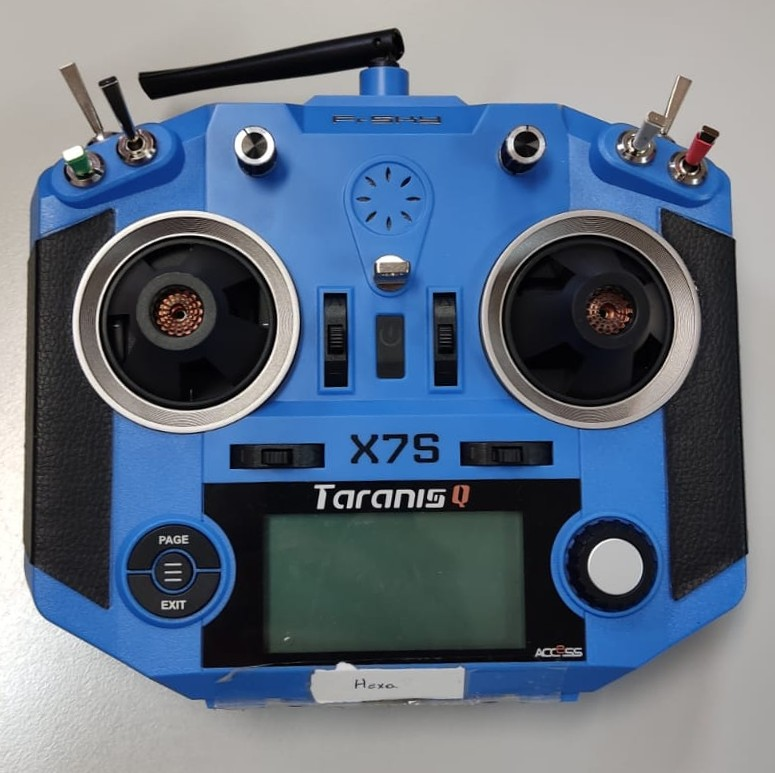
\includegraphics[width=0.65\textwidth]{imgs/02/taranis.jpg}}
\end{figure}

Las emisoras radiocontrol son un control remoto que permiten controlar la aeronave a distancia. La comunicación suele ser por radio frecuencia, ya que ofrecen más libertad de movimiento a la aeronave, aunque existen modelos que se comunican mediante cable con el dron (aeronaves en vuelo cautivo), y típicamente dúplex.
Las frecuencias utilizadas suelen depender de las necesidades de la aplicación. Esto es debido a que las características de la señal, fijan parámetros de la conexión tan importantes como el rango o el ancho de banda. Las bandas utilizadas se encuentran dentro de la frecuencia ultra-alta (UHF, \emph{Ultra High Frecuency}) sobre los 433MHz o sobre los 915MHz, en función la cantidad de datos que es necesario transmitir (mensajes, imágenes, vídeo, etc.). Otras frecuencias utilizas, aunque en menor medida debido a su corto alcance, son las bandas de 2.4GHz, correspondientes con el estándar WiFi (IEEE 802.11). La Figura \ref{fig:mod-telem} contiene un modulo receptor de telemetría a $2.4$GHz, listo para enlazar con la emisora mostrada.

\begin{figure}[ht]
 	\ffigbox[\FBwidth]{
 	    \caption[Módulo receptor \emph{FrSky X8R}]{Módulo receptor \emph{FrSky X8R}.}
 	    \label{fig:mod-telem}
 	}
 	{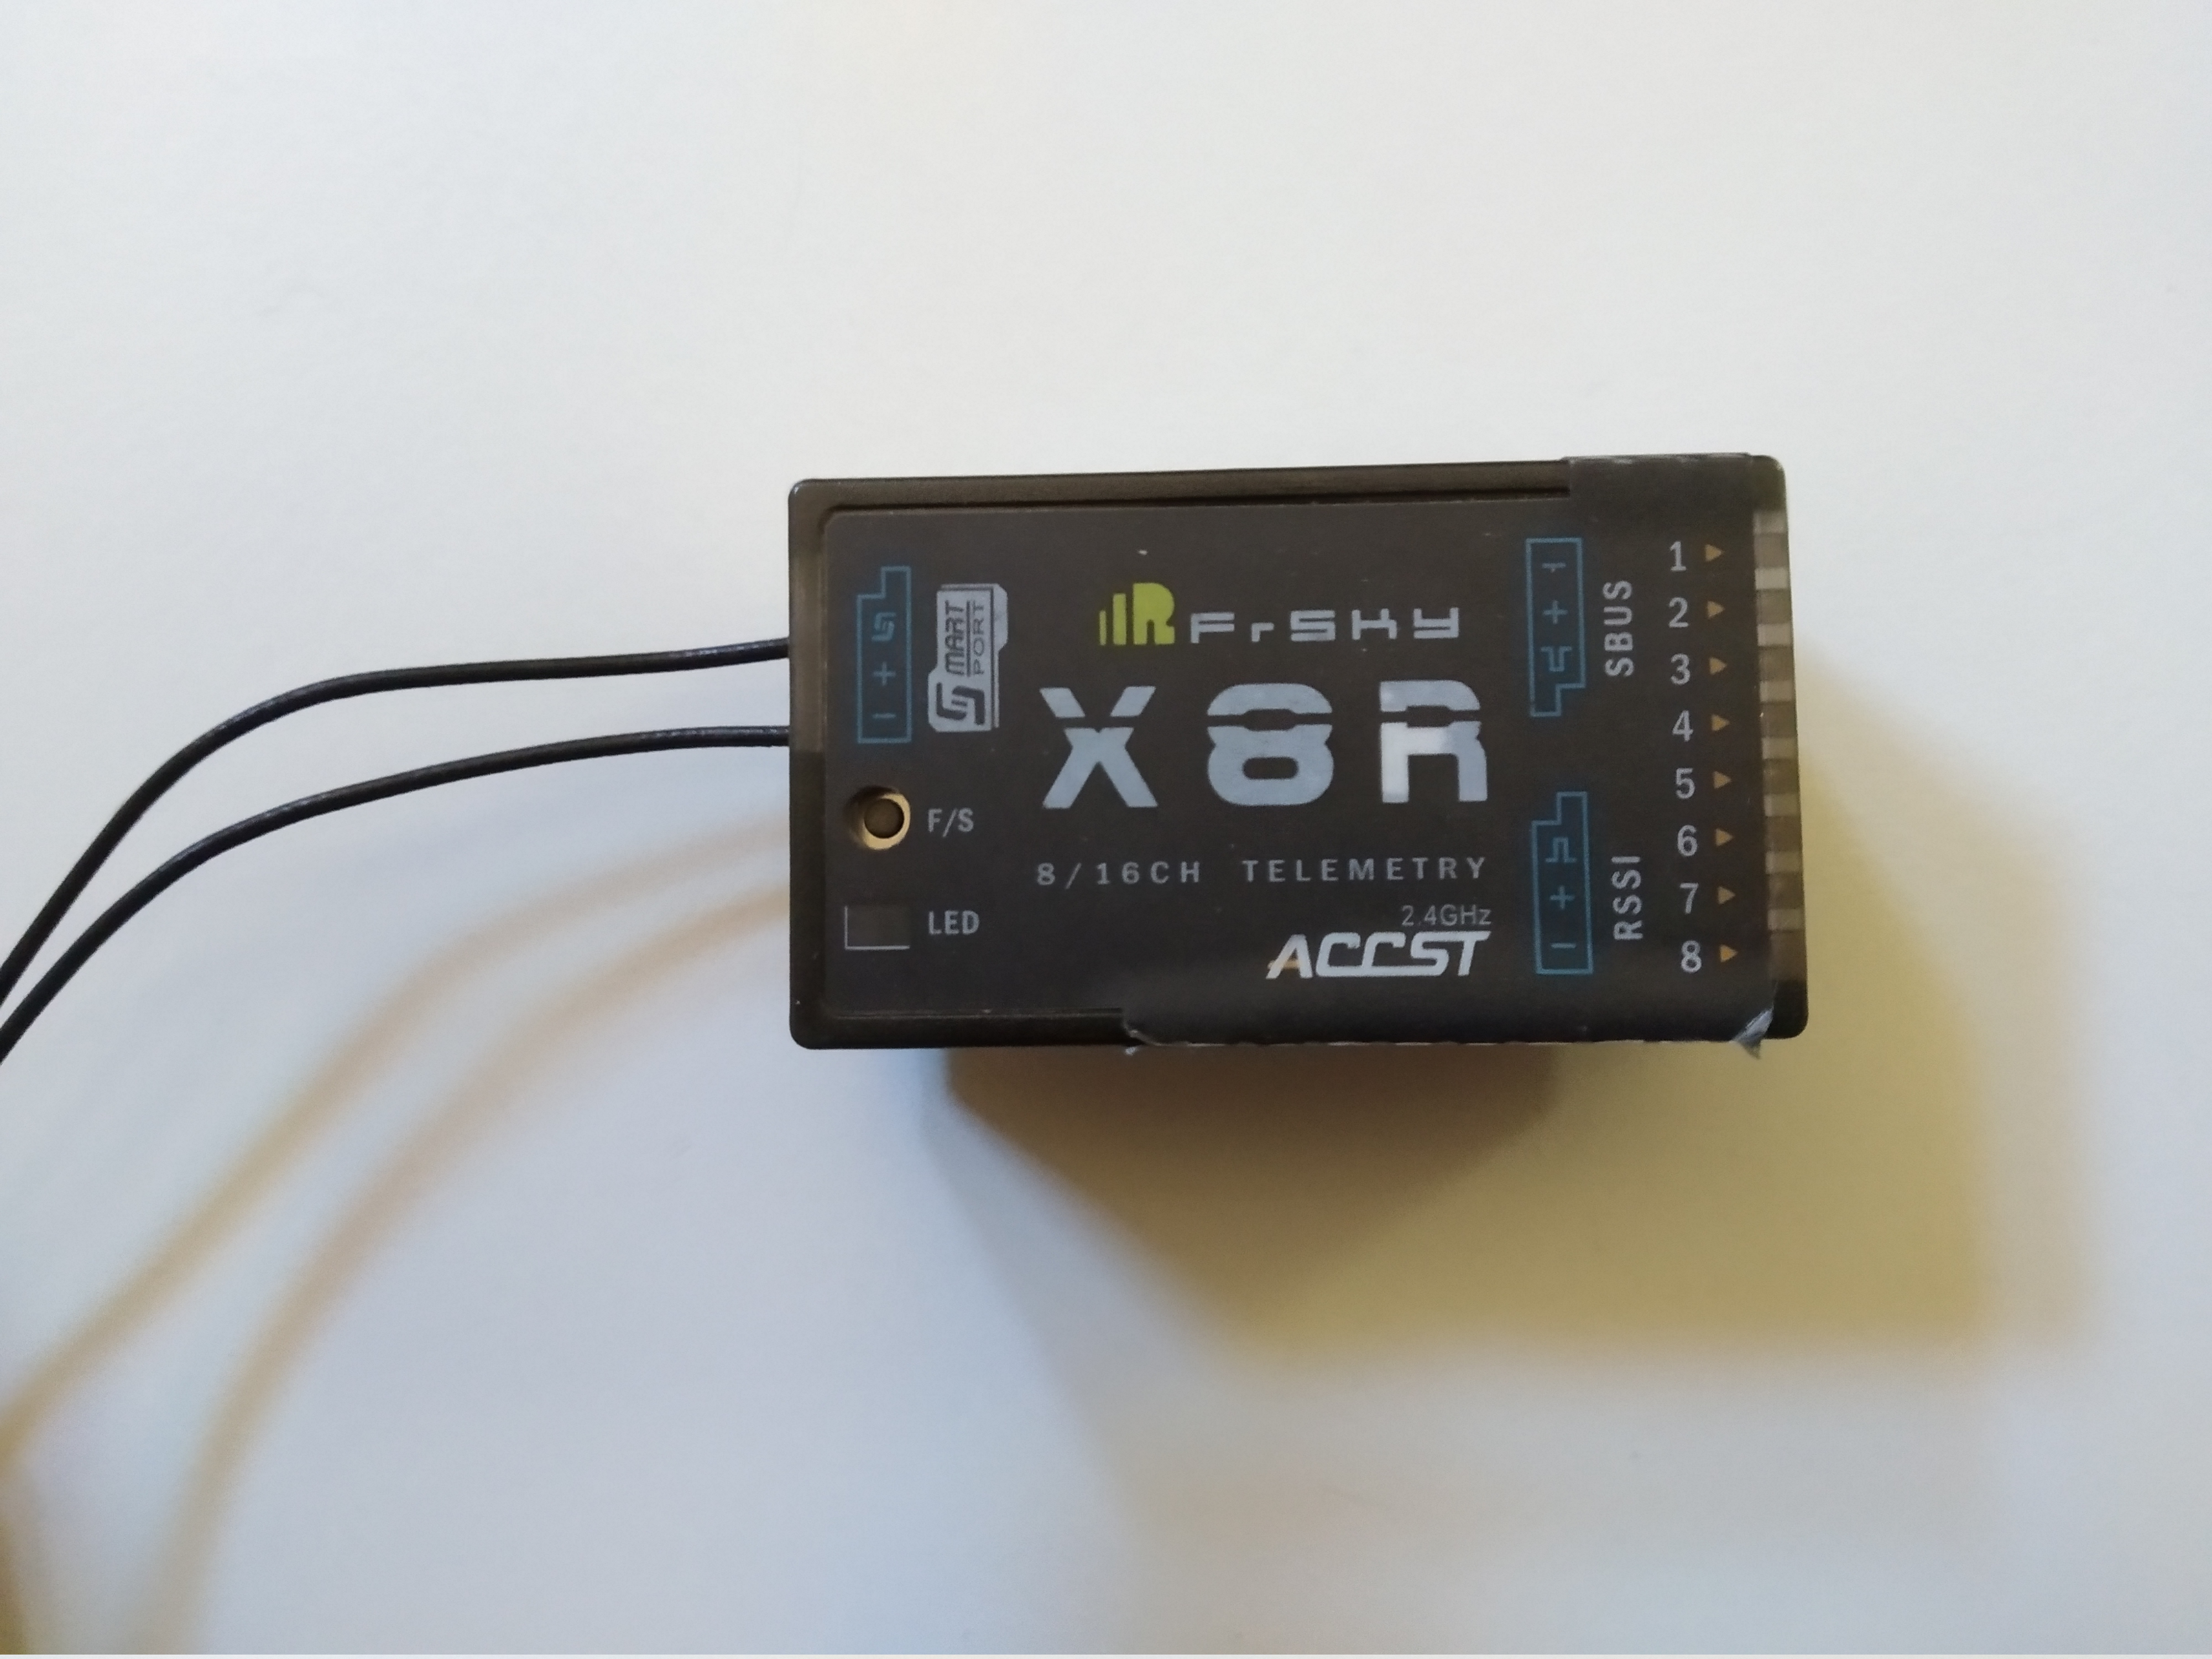
\includegraphics[width=0.55\textwidth]{02/frsky2.jpg}}
\end{figure}

Por otro lado, un ordenador ofrece una amplia variedad de aplicaciones con multitud posibilidades, desde aplicaciones generalistas a específicas a un ámbito (véase por ejemplo la topografía), o desde aplicaciones comerciales a libres o incluso desarrolladas por el propio usuario. \\
Debido a la gran cantidad de posibles opciones, los sucesivos apartados tratarán sobre diferentes tipos de aplicaciones que resultan relevantes para este proyecto.

\subsection{Estación de control terrestre} \label{section:herram-gcs}
Las Estaciones de Control Terrestre (GCS) son herramientas software que se utilizan para planificar y volar una misión. Generalmente proporcionan una pantalla con un mapa donde el usuario puede definir puntos de referencia para el vuelo y ver el progreso de la misión. Además, suelen disponer de una ``cabina virtual'', mostrando muchos de los mismos instrumentos que poseen los aviones tripulados.
Entre otras funcionalidades, suelen también disponer de herramientas de configuración de la aeronave y herramientas de descarga y análisis de archivos de registro de vuelo.

\begin{figure}[ht]
 	\ffigbox[\FBwidth] {
 	    \caption[QGroundControl]{QGroundControl.}
 	    \label{fig:qgcs}
 	}
 	{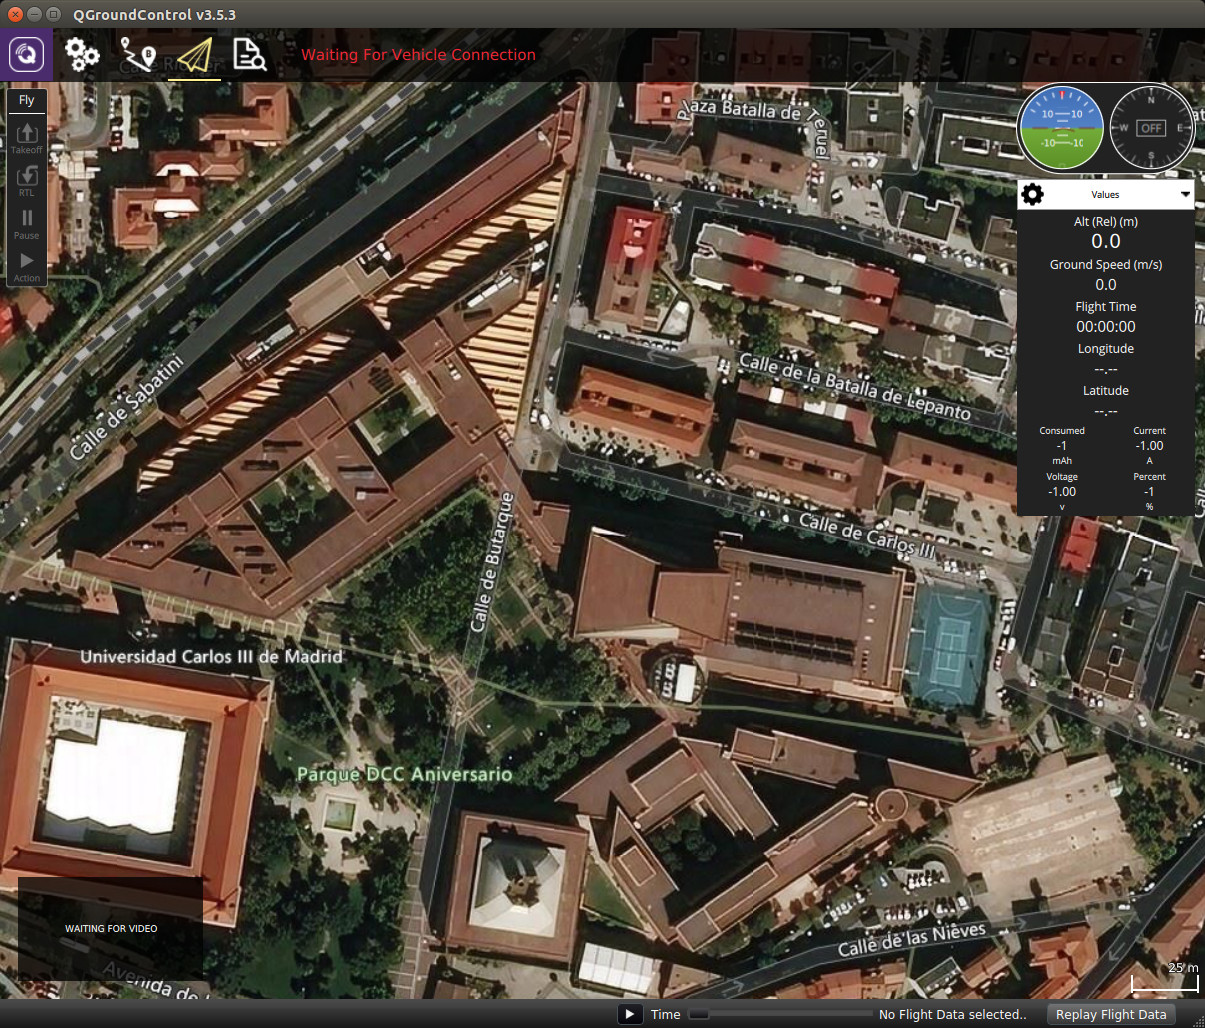
\includegraphics[width=0.75\textwidth]{02/qgcs.jpg}}
\end{figure}

Hoy en día, las principales GCS son, o bien software propietario de los principales fabricantes de UAVs, o software libre. Debido a su naturaleza, resultan más interesantes estas segundas. Entre ellas destacan principalmente \emph{QGroundControl} \cite{qgcs} y \emph{MissionPlanner} \cite{mission-planner}. La Figura \ref{fig:qgcs} muestra un ejemplo de estos programas en ejecución.

\subsection{Toolkits de vuelo} \label{section:herram-toolkits}
Los toolkits de vuelo incluyen bibliotecas, herramientas, drivers, etc para aplicaciones de vuelo programables. Ofrecen una interfaz de programación (API) que permite el desarrollo de aplicaciones a un nivel de abstracción muy elevado. Este tipo de software permite abstraerse de aspectos como el tipo concreto de aeronave o la comunicación con la misma. Cabe destacar que este tipo de software puede ejecutarse a bordo de la aeronave y formar parte del segmento aire o pertenecer al segmento tierra y ejecutarse en un ordenador externo. 

Un ejemplo de toolkit de vuelo es \emph{Aerostack} \cite{aerostack-github}. Aerostack ofrece a desarrolladores herramientas para diseñar y construir la arquitectura de control de sistemas robóticos aéreos, integrando múltiples soluciones computacionales heterogéneas como algoritmos de visión por ordenador, métodos de mapeo y auto-localización, planificadores de movimiento, etc. \cite{sanchez2016aerostack}. Ha sido desarrollada por el grupo de Visión por Computador y Robótica Aérea de la Universidad Politécnica de Madrid (CVAR-UPM) \cite{cvar} y actualmente se encuentra en su versión 5.

\section{Segmento aire} \label{section:herram-aire}
El lado aéreo consiste en la plataforma aérea, es decir el dron en si, junto a todos los elementos a bordo que componen el sistema. En esta sección se presentan dos tipos de aeronaves, reales o simuladas, que se abordarán los sucesivos apartados.

El elemento principal de una aeronave es el autopiloto, el cual se encarga del control de los actuadores y de la estabilización de vuelo y la navegación a través de los sensores. Un autopiloto se compone de una parte hardware (controladora) que va embarcada en la aeronave y una parte software (firmware) que se ejecuta en el hardware.
El funcionamiento que sigue una aeronave simulada es el mismo que el de una real. La Figura \ref{fig:loop-control} representa el bucle estándar de control disponible en los autopilotos más comunes.

\begin{figure}[ht]
 	\ffigbox[\FBwidth] {
 	    \caption[Bucle de control de un UAV]{Bucle de control de un UAV \cite{loop-control}.}
        \label{fig:loop-control}
 	}
 	{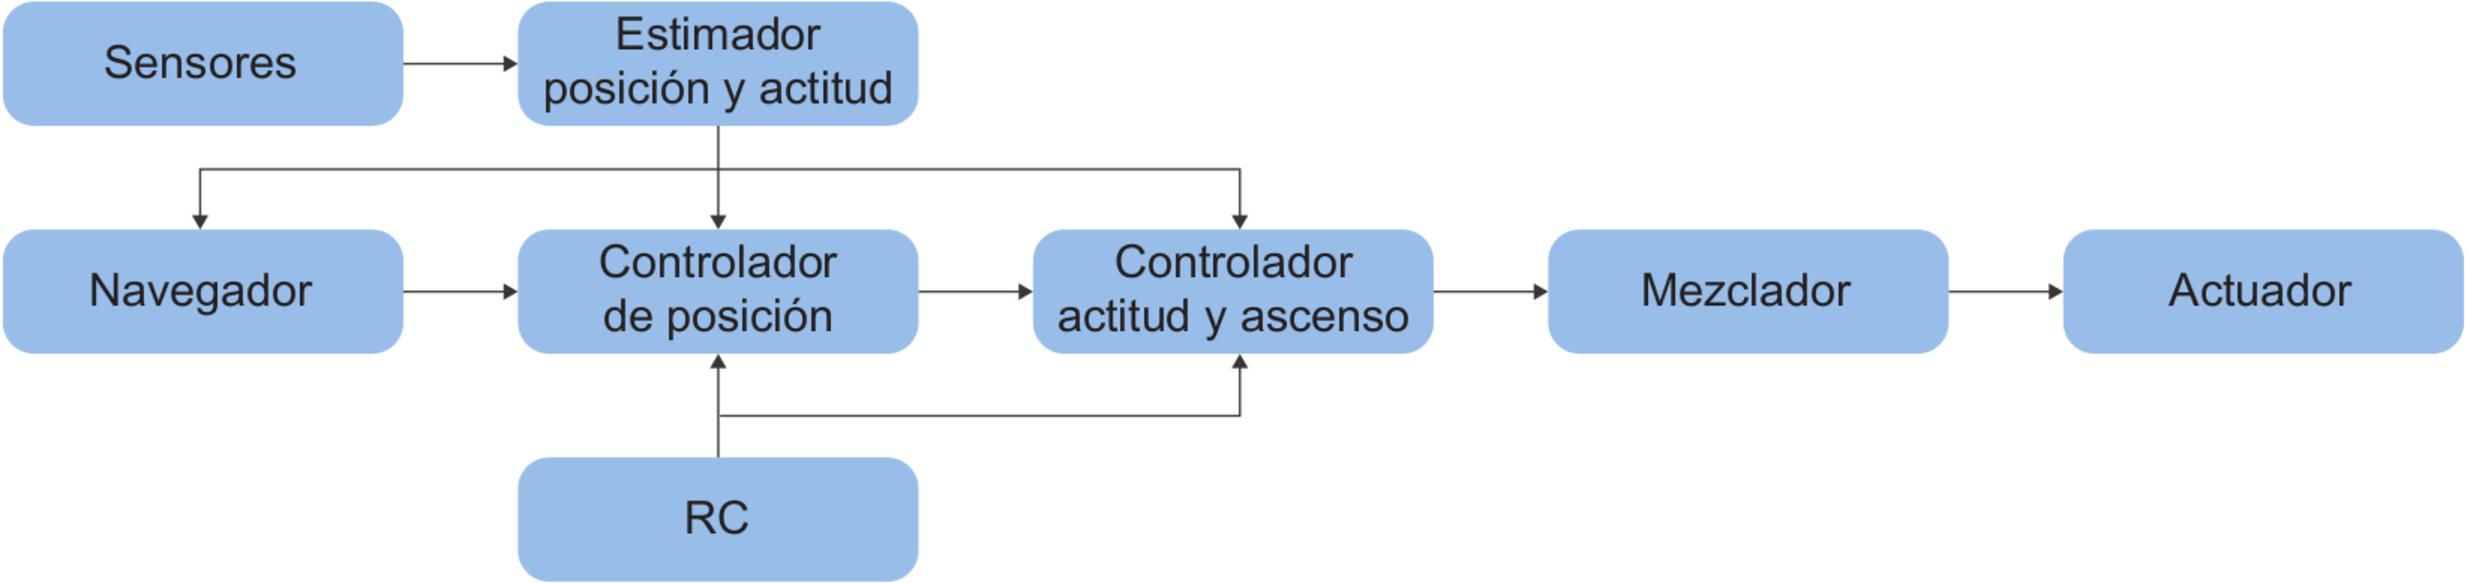
\includegraphics[width=\textwidth]{02/loop-control.pdf}}
\end{figure}

El funcionamiento de un bucle de control básico es el siguiente. El estimador toma una o más entradas de diferentes sensores, las combina y calcula el estado del vehículo. La controladora toma un punto de ajuste y una medición o estado estimado como entradas. Su objetivo es ajustar el valor del estado estimado de modo que coincida con el punto de ajuste. La salida es una corrección para eventualmente alcanzar ese punto de ajuste. Por ejemplo, el controlador de posición toma los puntos de ajuste de posición como entradas, y según la posición estimada calcula la salida que es un punto de ajuste de actitud y empuje que mueve el vehículo hacia la posición deseada. Finalmente, el mezclador toma comandos concretos, como girar a la derecha, y los traduce a comando de motor individuales, al tiempo que garantiza que no se excedan algunos límites. Esta traducción es específica para cada vehículo y depende de varios factores, como la disposición del motor con respecto al centro de gravedad o la inercia rotacional del vehículo, entre otros.

\subsection{Aeronaves reales} \label{section:herram-reales}
Existen multitud de aeronaves y diversas posibles clasificaciones, como la propuesta por Barrientos et al. (Fig. \ref{fig:clasif-uav}) \cite{barrientos2007vehiculos}. Otro posible criterio es la naturaleza del firmware, en base a sí es propietario o libre. En una aeronave libre el usuario tiene acceso a la controladora y al software de vuelo, que sería de código abierto y donde el mismo usuario podría modificar si lo precisa. En frente se encuentran las aeronaves propietarias, donde tanto la controladora y el firmware son privados y no accesibles al usuario. \\

\begin{figure}[ht]
    \ffigbox[\FBwidth]{
     	\begin{subfigure}{0.45\textwidth}
            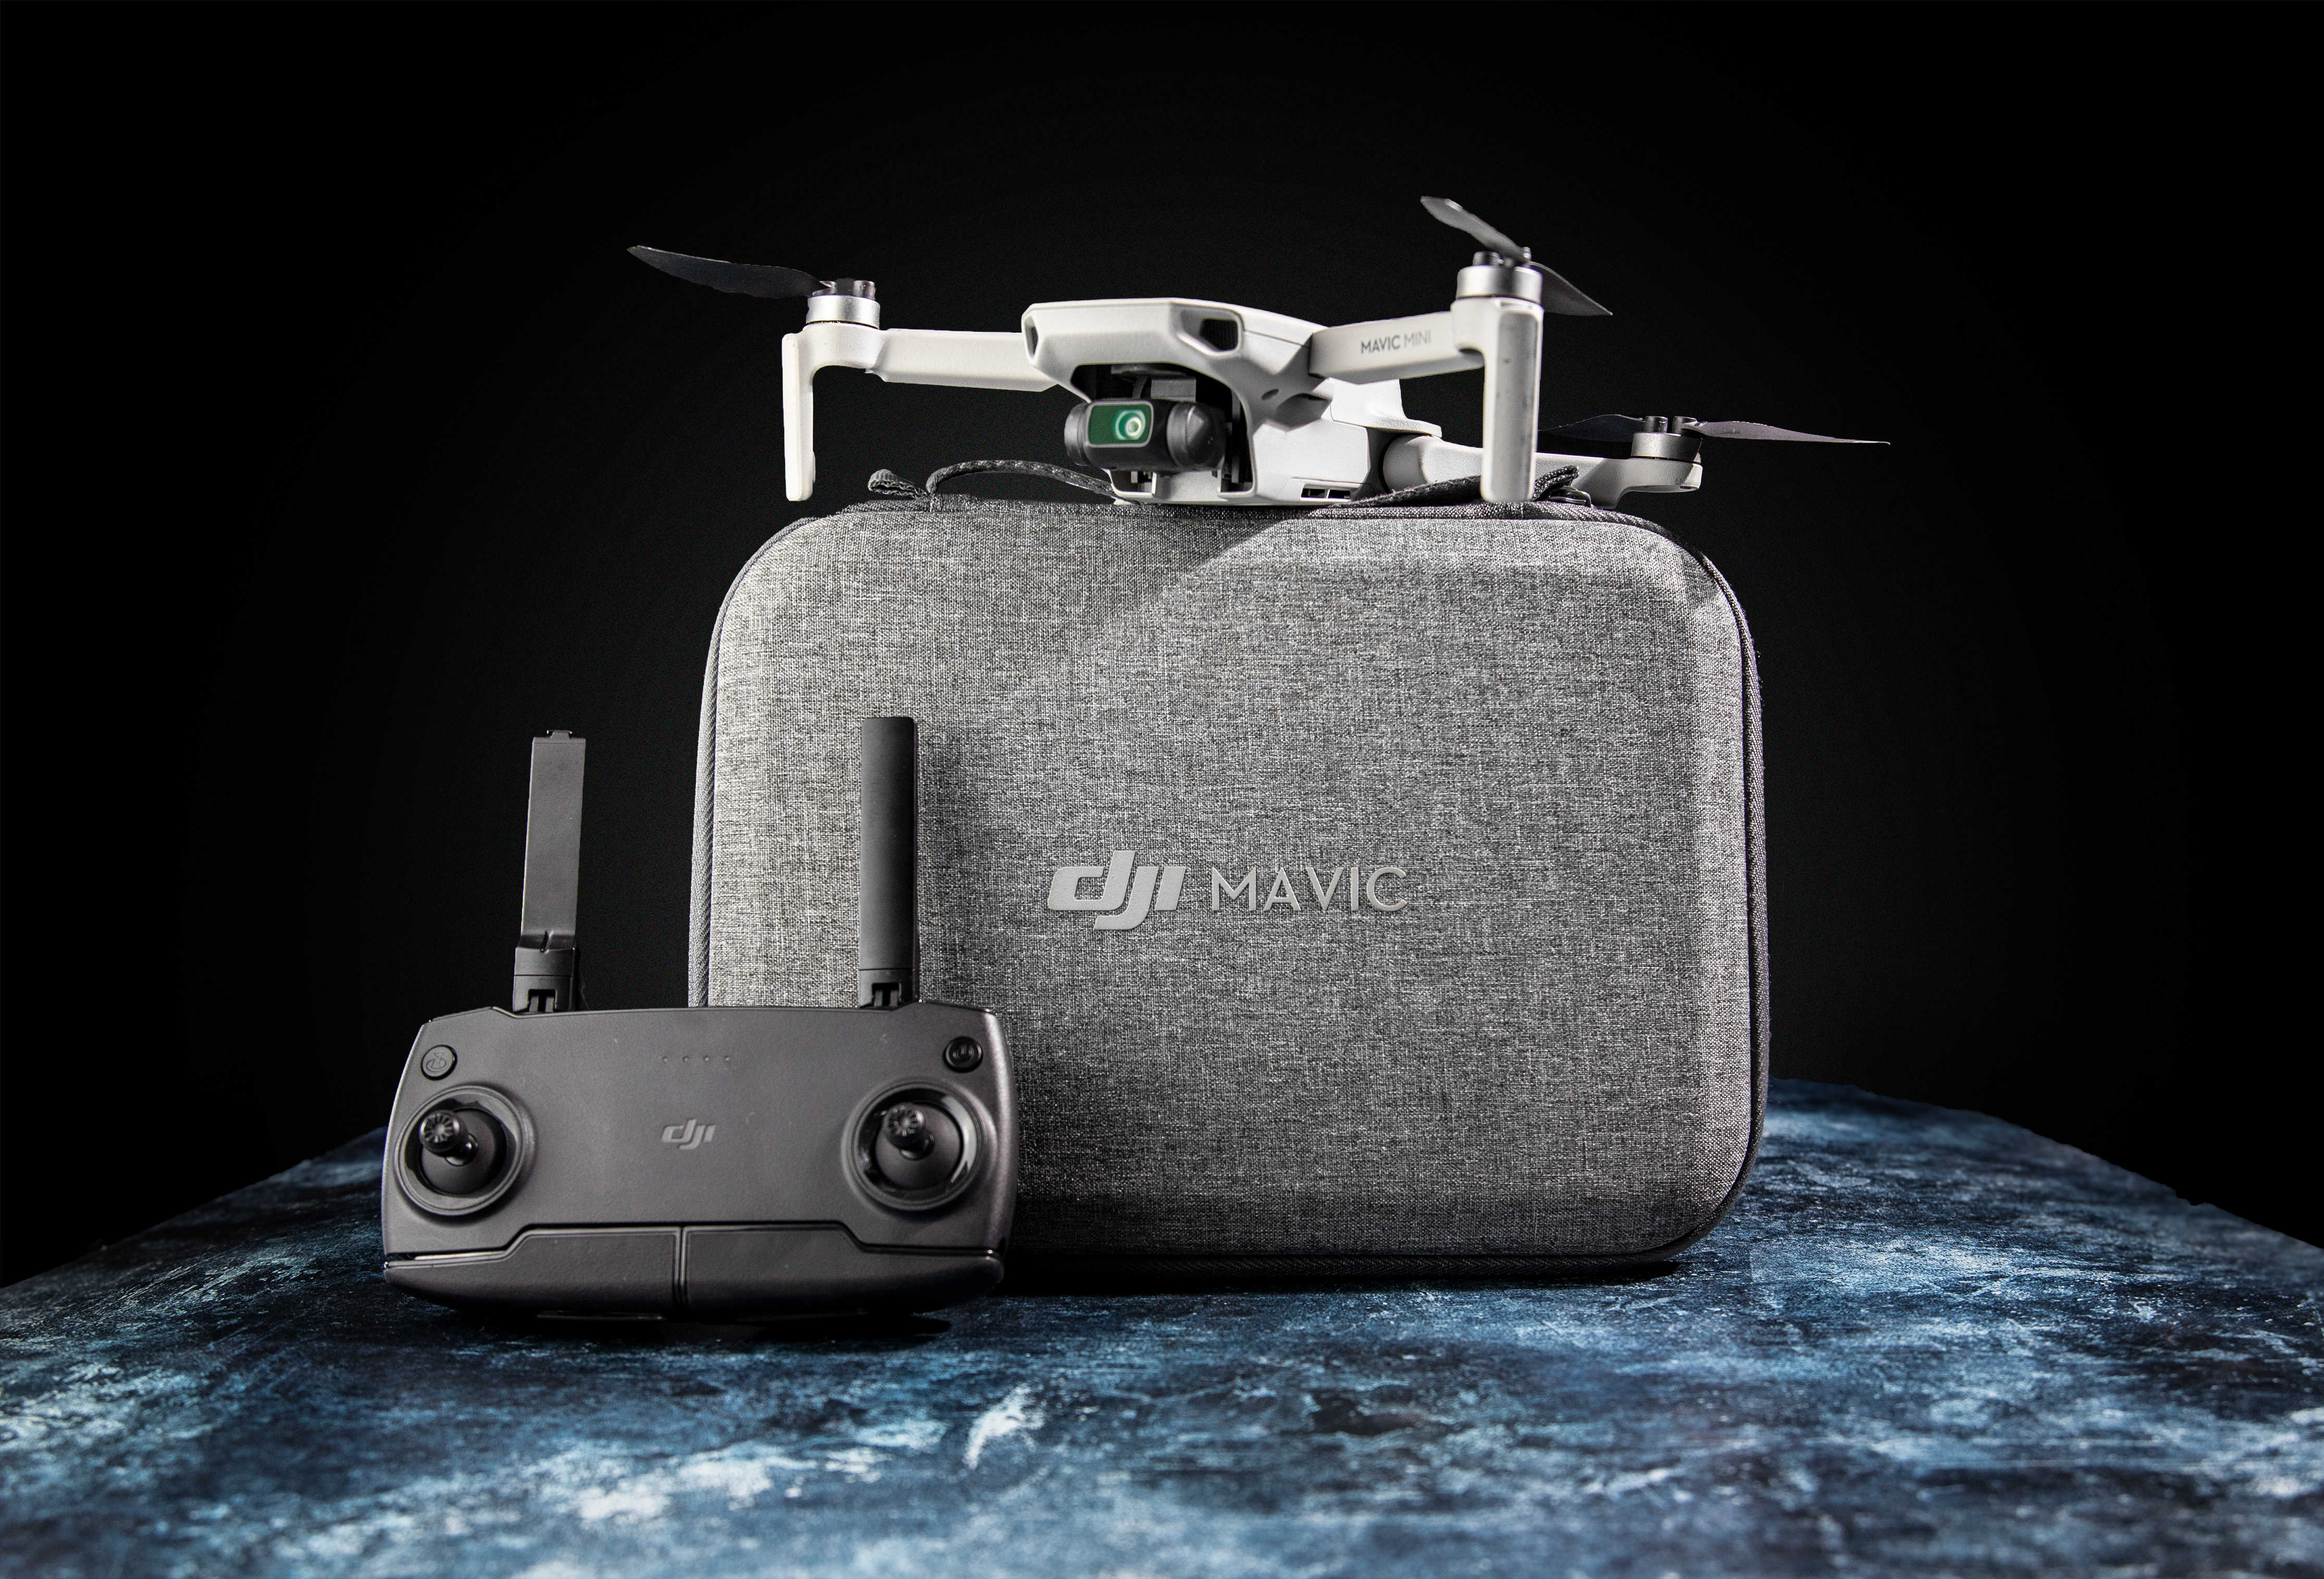
\includegraphics[height=4.5cm]{02/mavic.jpg}
            \caption{DJI Mavic.}
            \label{fig:dji-mavic}
        \end{subfigure}
        \begin{subfigure}{0.45\textwidth}
            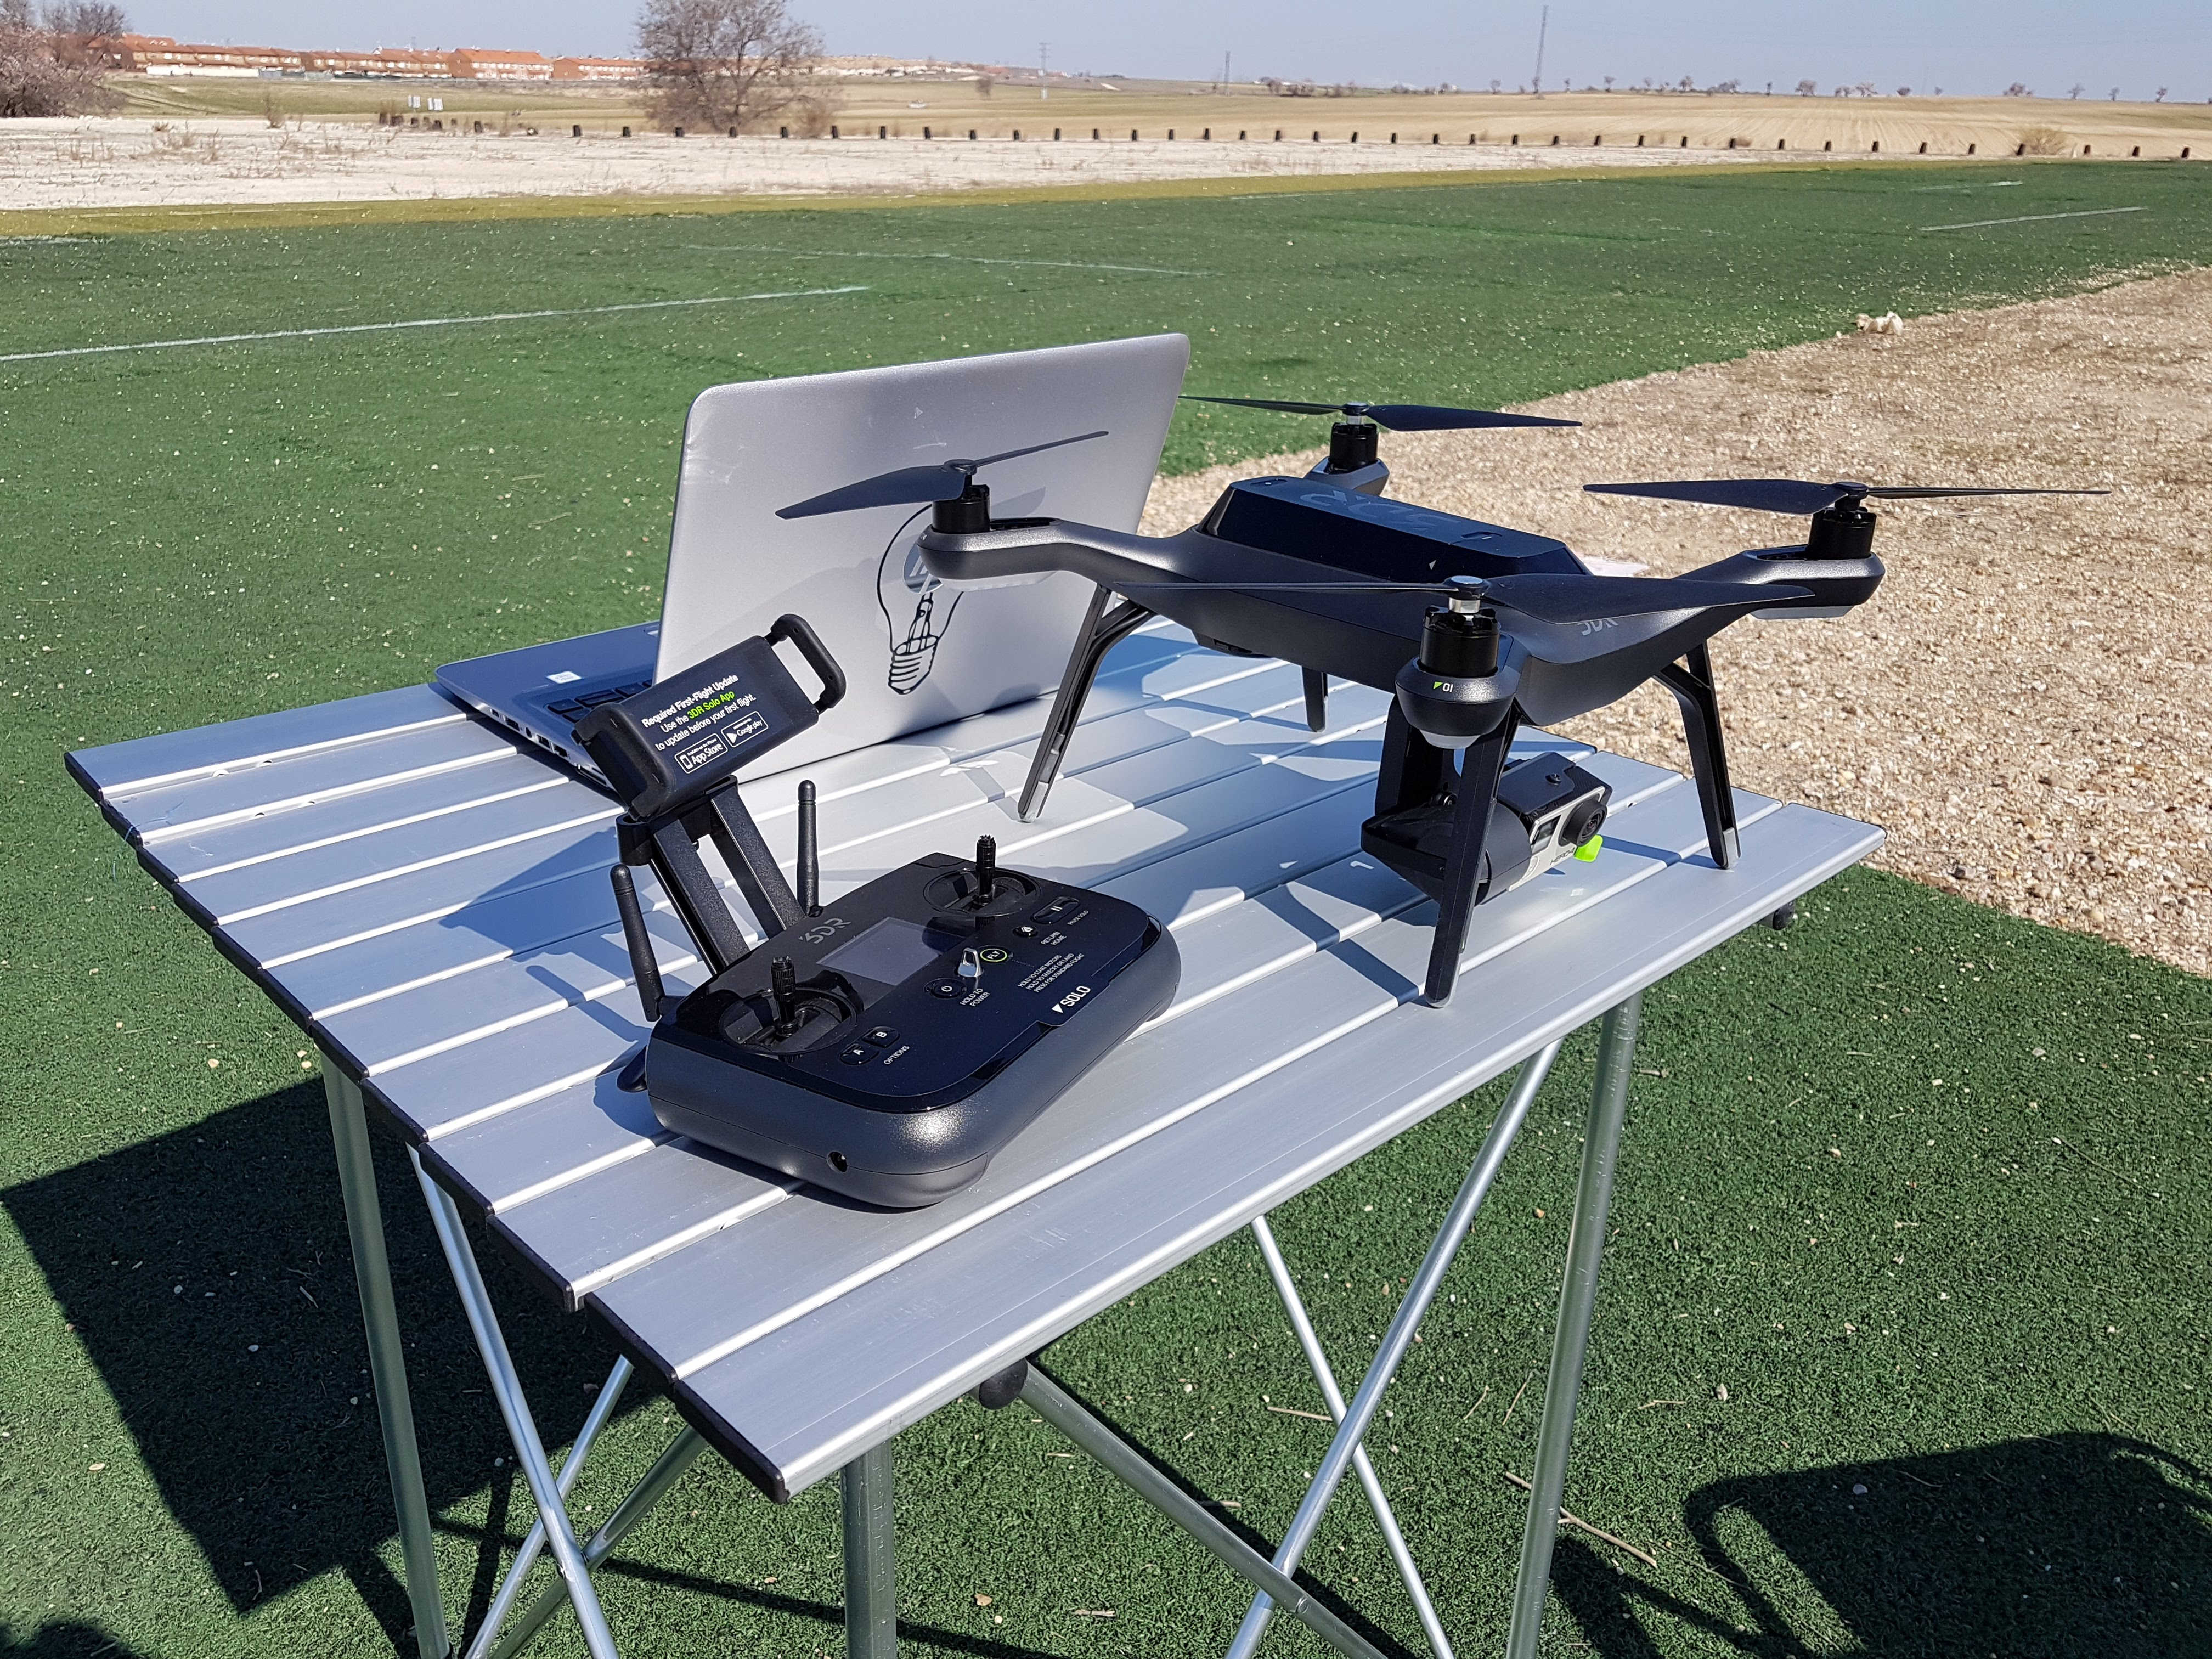
\includegraphics[height=4.5cm]{02/3dr.jpg}
            \caption{3DR Solo Drone.}
            \label{fig:3dr solo drone}
        \end{subfigure}
 	}{
 	    \caption[Ejemplos de drones de fabricantes propietarios]{Ejemplos de drones de fabricantes propietarios.}
        \label{fig:drone-prop}
    }
\end{figure}

Por un lado, entre los principales fabricantes propietarios se encuentran \emph{DJI} \cite{dji} o \emph{Parrot} \cite{parrot}, y hasta 2017 \emph{3DR Robotics} \cite{3dr} (ver Fig. \ref{fig:drone-prop}). \\
Por el otro lado, a la hora de hablar de plataformas libres es necesario distinguir entre los componentes hardware (principalmente la controladora) y el software de vuelo (firmware).

Los dos principales firmwares libres son \emph{PX4} y \emph{Ardupilot}.
PX4 es un software de control de vuelo de código abierto para drones y otros vehículos no tripulados. Proporciona un conjunto flexible de herramientas para que los desarrolladores compartan tecnologías que consigan crear soluciones personalizadas para aplicaciones de drones \cite{meier2015px4}. PX4 pertenece Dronecode, una organización sin ánimo de lucro de la Fundación Linux. \\
ArduPilot es un sistema de piloto automático confiable, versátil y de código abierto que admite muchos tipos de vehículos: multicópteros, helicópteros, aviones de ala fija, botes, submarinos, rovers y más \cite{ardupilot}. El código fuente está desarrollado por la comunidad abierta de desarrolladores \emph{Ardupilot-Dev Team}.

La principal controladora de vuelo utilizada con ambos firmware es \emph{Pixhawk} \cite{meier2011pixhawk}. Al igual que PX4, Pixhawk pertenece al grupo Dronecode.
La Figura \ref{fig:tipos-pix} contiene diferentes controladoras Pixhawk, mientras que la Figura \ref{fig:px4-real} muestra un multicóptero equipado con PX4.

% Figura Pixhawk 2.1 con descripción de componentes

\begin{figure}[ht]
 	\ffigbox[\FBwidth] {
     	\begin{subfigure}{0.45\textwidth}
            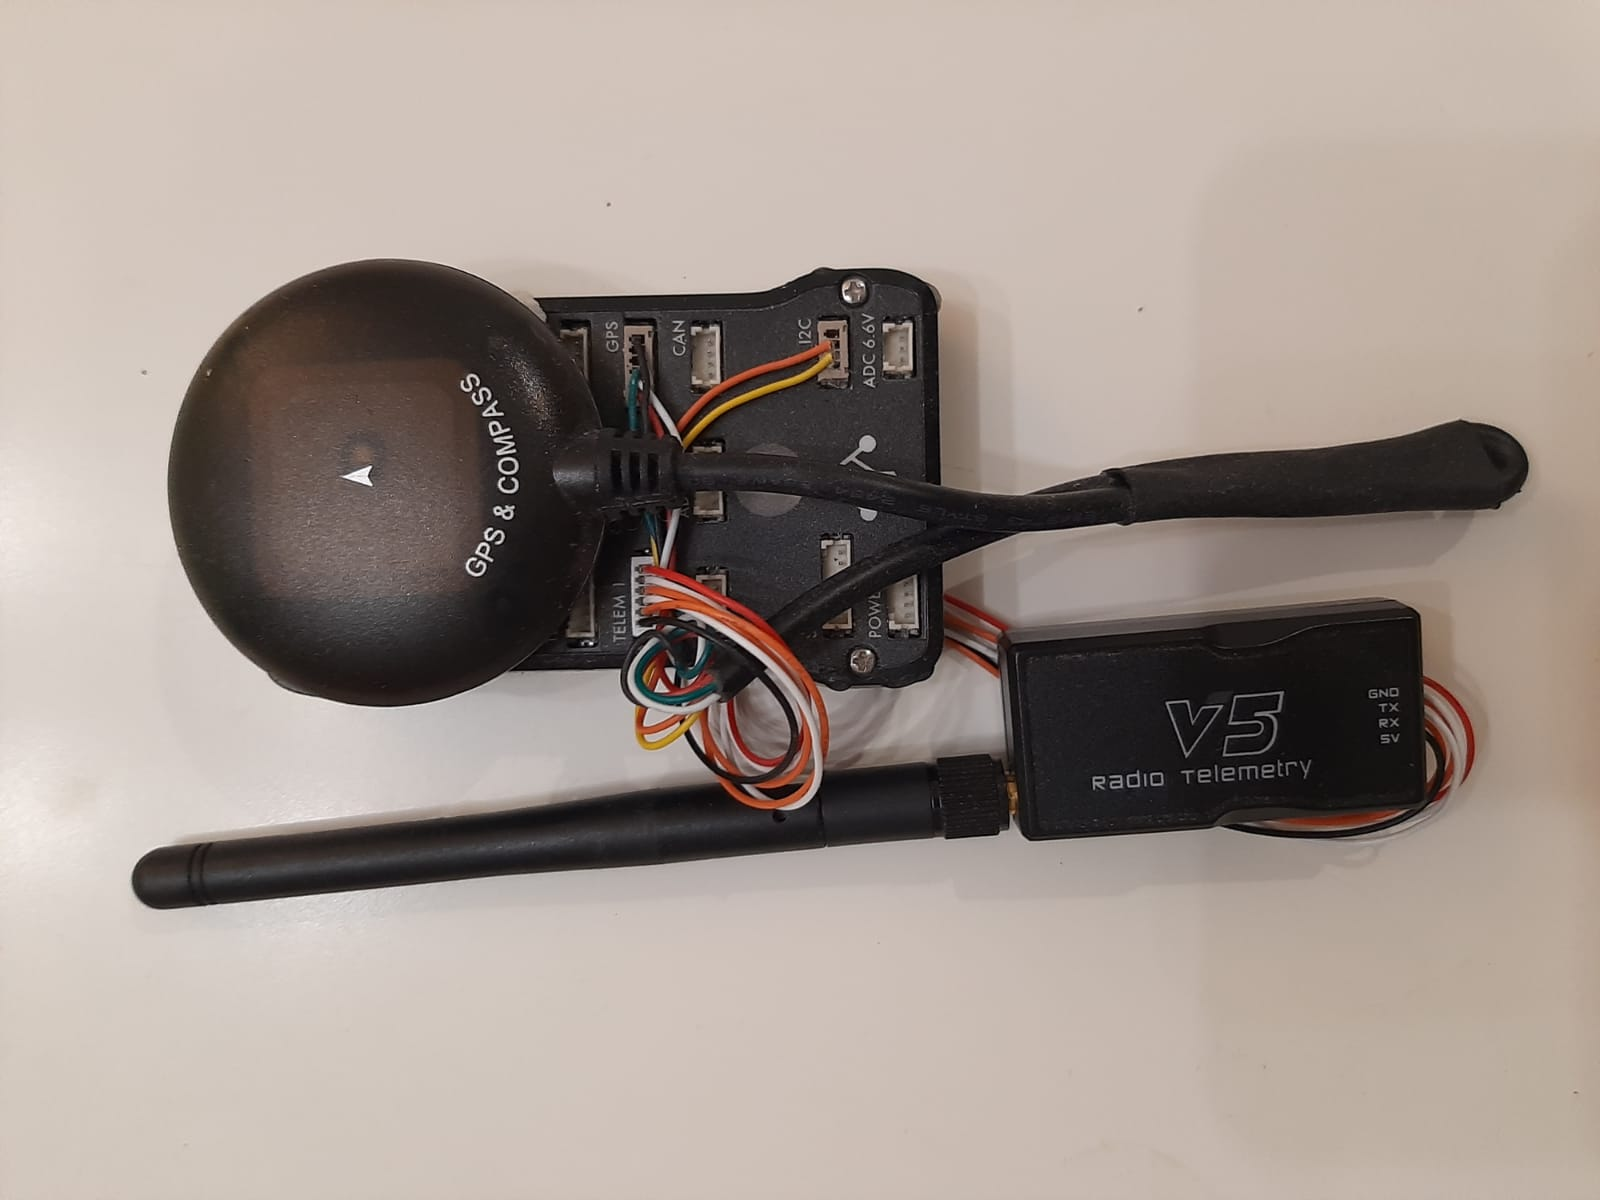
\includegraphics[height=5cm]{02/pixhawk.jpg}
            \caption{Pixhawk v1}
            \label{fig:pixh}
        \end{subfigure}
        \begin{subfigure}{0.45\textwidth}
            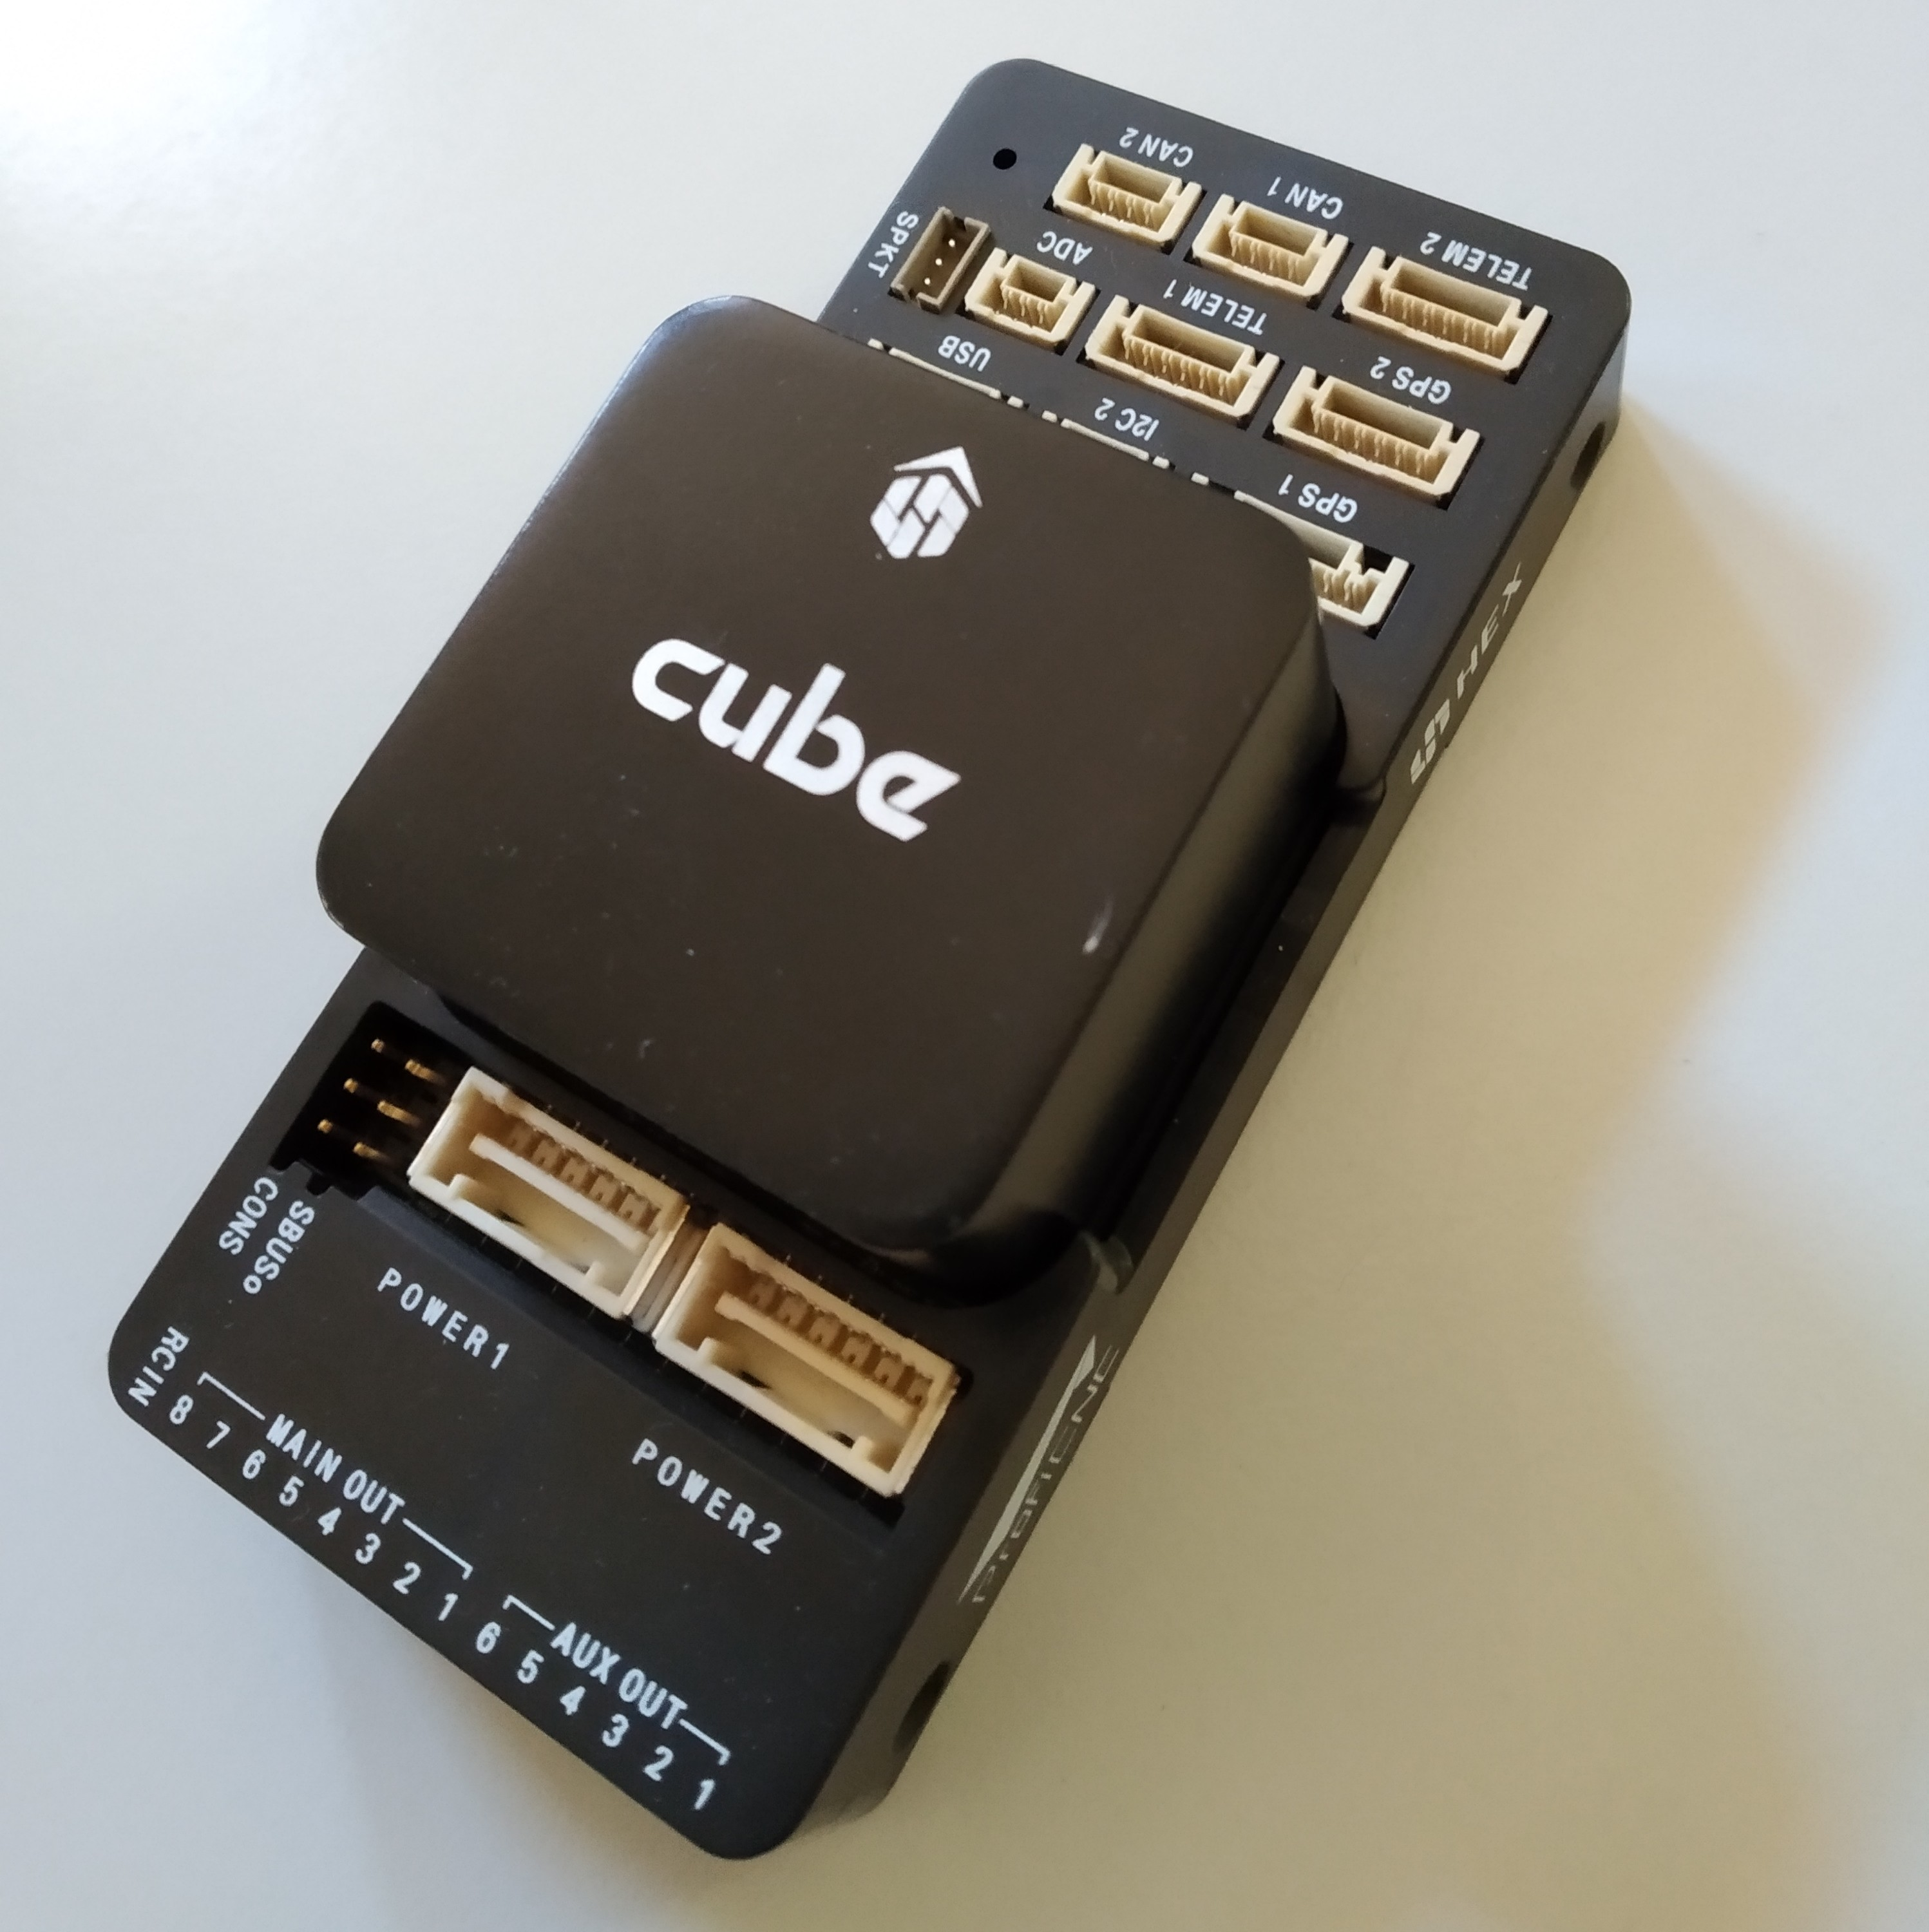
\includegraphics[height=6cm]{02/cube.jpg}
            \caption{Pixhawk v2 Cube}
            \label{fig:pixh2}
        \end{subfigure}
    }{
 	    \caption[Diferentes modelos de controladoras PixHawk]{Diferentes modelos de controladoras PixHawk.}
        \label{fig:tipos-pix}
 	}
\end{figure}

Existen diversos métodos para operar con UAS. Una primera clasificación posible es distinguir entre operaciones manuales o autónomas. Un vuelo manual dispone de un operario en tierra controlando a la aeronave a través de una emisora (control remoto), mientras que en un vuelo autónomo la aeronave puede realizar la misión de inicio a fin sin necesidad de un operador. Hoy en día, la forma más habitual de uso es operaciones semi-autónomas, con etapas en el vuelo en las que interviene el operario y otras en las que no.

\newpage
Los diferentes modos de operación se consiguen gracias a los modos de vuelo del autopiloto. Los modos de vuelo definen cómo responde el piloto automático a la entrada del control remoto y cómo gestiona el movimiento del vehículo durante un vuelo totalmente autónomo. \\
Los modos brindan diferentes niveles de asistencia al piloto, que van desde la automatización de tareas comunes como el despegue y el aterrizaje, hasta mecanismos que facilitan recuperar el nivel de vuelo, mantener el vehículo en una ruta o posición fija, etc. \\
En general, existen dos tipos de modos de vuelo, manuales y autónomos. Los manuales son aquellos en los que el piloto tiene el control sobre el vehículo a través del control remoto o emisora, mientras que los modos autónomos son aquellos que están totalmente controlados por el autopiloto. \\
Cobran gran interés estos últimos, pues no requieren ninguna entrada del control remoto. PX4 posee 6 modos autónomos, \emph{HOLD} (mantener posición actual), \emph{RETURN} (retorno al punto de despegue), \emph{MISSION} (vuelo de una misión preprogramada), \emph{TAKEOFF} (despegue), \emph{LAND} (aterrizaje), \emph{FOLLOW ME} (seguimiento mediante comandos de posición, solo disponible para multicópteros) y \emph{OFFBOARD} (control robótico) \cite{px4-flight-modes}. \\
Todos los modos salvo el último, \emph{OFFBOARD}, utilizan un control mediante posición GPS. De hecho el modo común de operación es el modo \emph{MISSION}, donde previo al vuelo al dron se le indica una secuencia de puntos de paso que sigue una vez en el aire gracias a la ayuda del sensor GPS de forma autónoma. Sin embargo, este tipo de vuelos solo es posible en exteriores y bajo cobertura GPS. En interiores no es posible al no disponer de cobertura GPS debido a limitaciones con la señal. \\
Así pues, el modo de operación en interiores, y en general en aplicaciones de robótica, es el modo \emph{OFFBOARD}. Este modo de vuelo permite un control variado de la aeronave, permitiendo no solo controlar a la aeronave mediante posición, sino también con comandos de velocidad, de aceleración o de fuerza.

\subsection{Aeronaves simuladas} \label{section:herram-sim}
Las aeronaves simuladas suelen utilizar software de vuelo libre, dada la naturaleza abierta del mismo. En una simulación, la parte física de la aeronave se ve sustituida por software (SITL, \emph{Sotfware-In-The-Loop}). El SITL es, en si mismo, un simulador. Contiene el software de vuelo y permite enviar y recibir comandos de vuelo sin necesidad de tener una controladora real, haciendo de intermediario entre el autopiloto y el modelo SDF, necesario en la visualización gráfica. Existen diferentes SITL en función del controlador simulado (PX4, ArduPilot, etc.) y en general suelen soportar la simulación de sensores sencillos como GPS, IMU, etc.

Dichas simulaciones se suelen acompañar de una visualización gráfica. Para ello, es necesario el uso de un simulador como \emph{Gazebo} \cite{gazebo}, \emph{AirSim} \cite{airsim} o \emph{jMAVSim} \cite{jmavsim}. El más extendido, debido a sus grandes prestaciones y posibilidades de configuración es Gazebo. \\
Simuladores como estos, permiten probar rápidamente algoritmos, diseñar robots o realizar pruebas sobre sistemas de inteligencia artificial sobre entornos realistas. Ofrecen funciones punteras como la simulación con precisión de poblaciones de robots en entornos complejos de interior y exterior, manteniendo un motor de físicas robusto y con gráficos configurables.
La Figura \ref{fig:drone-sim} muestra un dron simulado mediante jMAVsim con PX4 como autopiloto. 

\begin{figure}[ht]
 	\ffigbox[\FBwidth] {
 	    \caption[Dron simulado mediante jMAVsim]{Dron simulado mediante jMAVsim.}
        \label{fig:drone-sim}
 	}
 	{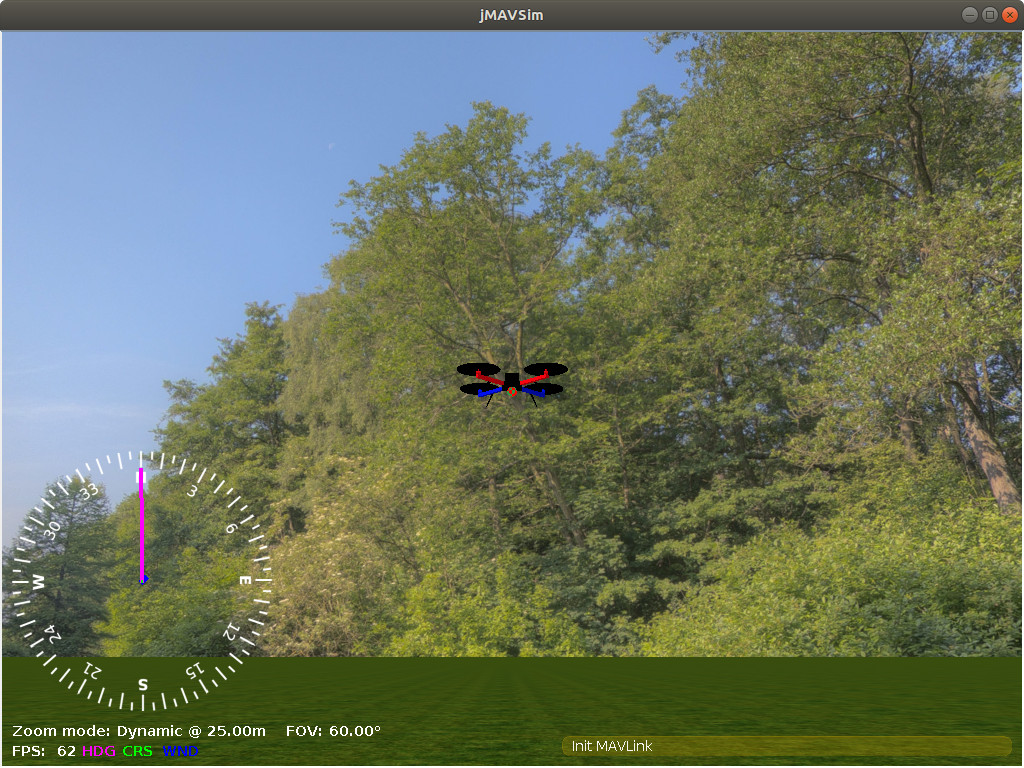
\includegraphics[width=0.90\textwidth]{02/jmavsim.jpg}}
\end{figure}

\section{Protocolo de comunicaciones} \label{section:herram-protocolo}
El protocolo de comunicaciones puede ser propietario, utilizado por fabricantes de aeronaves y diferentes para cada una de ellas, o libre. El protocolo de comunicaciones libre por excelencia es MAVLink \cite{mavlink}, que se ha convertido \emph{de facto} en el estándar del sector. \\
MAVLink son las siglas de \emph{Micro Air Vehicle Link}, un protocolo de comunicaciones muy ligero para el intercambio de mensajes con un dron y sus componentes a bordo. MAVLink se sitúa entre los extremos de la comunicación, siendo el puente de comunicación entre el lado tierra y el lado aire. Es considerado como el protocolo estándar de comunicaciones en robótica aérea y multitud soluciones comerciales lo utilizan, por ejemplo las ya mencionadas GCS, \emph{QGroundControl} y \emph{Mission Planner}.

El protocolo se compone de cuatro tipo de elementos: mensajes, comandos, enumerados y microservicios. \\
Los mensajes son el objeto más pequeño de intercambio de información del protocolo. Sirven para transmitir el estado o información de la aeronave, principalmente datos de navegación o de posición.
Son muchos los mensajes existentes y de diversa utilidad, como se puede comprobar en la documentación existente \cite{mavlink-msg}. Ejemplo de ello son los mensajes \emph{HEARTBEAT} (ver Cód. \ref{lst:heartbeat}) o \emph{ATTITUDE}.

\lstinputlisting[caption={Definición del mensaje HEARTBEAT de MAVLink.}, language=xml, captionpos=b, label={lst:heartbeat}]{code/heartbeat.xml}

\newpage
Los comandos sirven para transmitir peticiones y acciones a la aeronave desde la GCS, o viceversa. Se encapsulan en un tipo especial de mensajes (\emph{COMMAND\_INT} o \emph{COMMAND\_LONG}). Los comandos pueden ser de tres tipos: de navegación, de acción y de condición, en función del tipo de petición requerida. Los comandos utilizados en el protocolo se pueden comprobar también en la documentación de MAVLink \cite{mavlink-msg}. 
El Código \ref{lst:cmd} muestra, a modo de ejemplo, la estructura de un comando de navegación a un punto.

Los enumerados describen diferentes estados, como puede ser el modo de vuelo, el tipo de aeronave o el estado de la comunicación, y son usados como campos de los mensajes o de los comandos. Los enumerados sirven, en definitiva, para representar errores, estados o modos. Cada enumerado tiene un atributo de nombre obligatorio y puede contener una serie de elementos de entrada (con nombres exclusivos de enumeración) para los valores admitidos. \\
En el mensaje HEARTBEAT (Cód. \ref{lst:heartbeat}) se hace referencia a varios, como \emph{MAV\_TYPE} o \emph{MAV\_AUTOPILOT}. Al igual que los mensajes y los comandos, los enumerados disponibles se pueden comprobar en la documentación de MAVLink \cite{mavlink-msg}.

\lstinputlisting[caption={Definición CMD\_NAV\_WAYPOINT, comando de MAVLink.}, language=xml, captionpos=b, label={lst:cmd}]{code/cmd.xml}

Por último, los microservicios establecen cómo deben ser intercambiados los mensajes y comandos para un correcto funcionamiento de la comunicación. Representan protocolos de alto nivel que los sistemas MAVLink pueden adoptar para una mejor interacción. \\
Los microservicios se utilizan para intercambiar muchos tipos de datos, incluidos: parámetros, misiones, trayectorias, imágenes y otros archivos. Los datos pueden ser mucho más grandes de lo que cabe en un solo mensaje, por lo que los microservicios definirán cómo se dividen y se vuelven a ensamblar los datos, y cómo garantizar que los datos perdidos se vuelvan a transmitir. Otros microservicios proporcionan reconocimiento de comandos, informes de errores, etc. Los diferentes microservicios se definen en la documentación de MAVLink \cite{mavlink-microserv}.

\begin{table}[H]
	\ttabbox[\FBwidth]
	{\caption{Principales mensajes de MAVLink.} \label{tab:mavlink}}
	{\begin{tabular}{|c|c|}
		\multicolumn{2}{c}{\textbf{MENSAJES}} \\
		\hline
		HEARTBEAT           & VFR\_HUD  \\
		\hline
        SYS\_STATUS         & SET\_MODE \\
        \hline
        HIGHRES\_IMU        & RADIO\_STATUS     \\
        \hline
        BATTERY\_STATUS     & ATTITUDE  \\
        \hline
        \multicolumn{2}{|c|}{GLOBAL\_POSITION\_INT}  \\ 
        \hline
		\multicolumn{2}{l}{Fuente: MAVLink \cite{mavlink}}
	\end{tabular}}
\end{table}

Comandos como el presentado (Cód. \ref{lst:cmd}) son útiles a la hora navegar de forma tradicional mediante posición GPS. Junto a este comando, otros mensajes y comandos son necesarios para un correcto funcionamiento del protocolo de comunicaciones. La Tabla \ref{tab:mavlink} recoge varios mensajes muy utilizados.

\section{Programación de robots}
Existen multitud de herramientas que permiten y facilitan la programación de robots. Esta sección se centra en dos, las plataformas robóticas de software y los algoritmos de aprendizaje profundo. 

\subsection{Plataformas robóticas de roftware} \label{section:herram-rob-platf}
Las plataformas robóticas de software son entornos que permiten la interacción software-hardware. Una analogía que las define con sencillez es que si los datos son el torrente sanguíneo de tu robot, entonces las plataformas robóticas de software son el sistema circulatorio del mismo. \\
Más específicamente, estas plataformas permiten la construcción de sistemas de control de robots como una colección de programas que se comunican \emph{peer-to-peer} con una familia extensible de tipos de conexión. A este tipo de plataformas se les conoce comúnmente como \emph{middleware}, al encontrarse a medio camino entre el hardware y el software. \\
Pese a describir este software como parte del segmento tierra, es importante destacar que puede también pertenecer al segmento aire, en función de donde esté ubicado.
Existen múltiples plataformas robóticas, las más comunes son ROS \cite{quigley2009ros}, YARP \cite{fitzpatrick2014middle, metta2006yarp}, Orocos \cite{bruyninckx2001open} o CARMEN \cite{montemerlo2003perspectives}.

Hoy en día, la plataforma más utilizada en robótica es ROS. ROS (\emph{Robot Operating System}) es ``un meta-sistema operativo de código abierto para su robot'', mantenido por \emph{Open Source Robotics Foundation} (OSRF) \cite{osrf}. A pesar del nombre, ROS no es un sistema operativo al uso. Más bien, es un SDK (\emph{Software Developer Kit}, kit de desarrollo de software) que proporciona los componentes básicos para crear aplicaciones robóticas.

Principalmente, ROS proporciona un sistema de envío de mensajes, \emph{middleware}. El sistema de mensajería permite la comunicación entre nodos distribuidos, típicamente, a través de un patrón anónimo de publicación/subscripción a \emph{topics}. El enfoque de ROS da como resultado sistemas más fáciles de mantener, contribuir y reutilizar. \\
Además, ROS proporciona servicios que se esperarían de un sistema operativo, incluyendo abstracción de hardware, control de dispositivos de bajo nivel, implementación de funcionalidades comunes o manejo de paquetes. Otra funcionalidad relevante son una serie de librerías y herramientas de desarrollo. Herramientas para el lanzamiento, la introspección, la depuración, la visualización, el graficado o la grabación y reproducción de ejecuciones.

El ecosistema de ROS es enorme. Actualmente, soporta multitud de robots y sensores, y está integrado en los principales simuladores como Gazebo. Además, otra gran ventaja es la comunidad alrededor de ROS, la cual es global y de gran tamaño, lo que produce que haya gran cantidad de documentación disponible.

\subsection{Aprendizaje profundo}
El aprendizaje profundo es un conjunto de algoritmos de aprendizaje automático que intenta modelar abstracciones de datos de alto nivel usando redes neuronales. Las redes neuronales son arquitecturas computacionales de datos expresados en forma matricial o tensorial. Cada unidad, llamada \emph{neurona}, se organiza en capas que forman la red.

\begin{figure}[ht]
 	\ffigbox[\FBwidth] {
 	    \caption[Arquitectura perceptrón multicapa]{Arquitectura perceptrón multicapa.}
 	    \label{fig:mlp}
 	}
 	{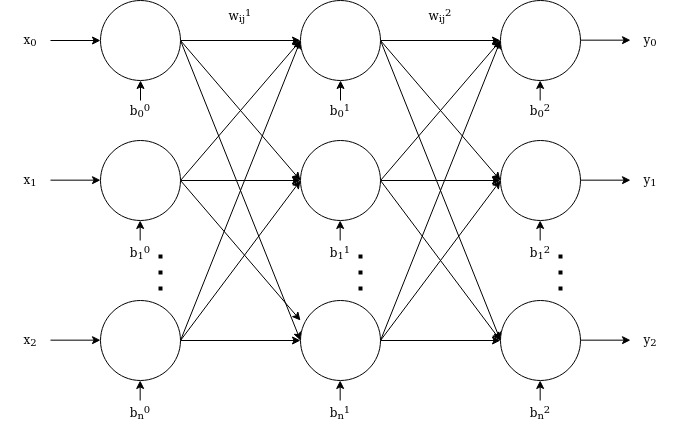
\includegraphics[width=0.75\textwidth]{02/mlp.jpg}}
\end{figure}

La palabra ``profundo'' hace referencia al número de capas que posee la red, siendo redes profundas aquellas redes con más de tres capas. En la Figura \ref{fig:mlp} se ilustra una arquitectura de red neuronal básica, conocida como perceptrón multicapa (MLP, \emph{MultiLayer Perceptron}). La arquitectura presentada posee una capa de entrada, una de salida y una capa oculta.

Existen diferentes marcos de programación que permiten el desarrollo redes y algoritmos. Las principales plataformas son Keras \cite{keras}, TensorFlow \cite{tensorflow}, PyTorch \cite{pytorch} y, en el ámbito de la visión, Darknet \cite{darknet13}.

\begin{itemize}
    \item \textbf{Keras} es una biblioteca de redes neuronales de código abierto escrita en Python y desarrollada por François Chollet. Es capaz de ejecutarse sobre TensorFlow (fue integrado a mediados de 2017) y otros marcos de programación. Está diseñado para permitir una experimentación rápida con redes neuronales profundas.
    \item \textbf{TensorFlow} es una biblioteca de software de código abierto para la programación de redes neuronales y del flujo de datos en una variedad de tareas, desarrollado por Google y lanzado en 2015. Ofrece múltiples niveles de abstracción para construir y entrenar modelos.
    \item \textbf{PyTorch} es una biblioteca de aprendizaje automático de código abierto para Python, basada en Torch. Se utiliza para aplicaciones como el procesamiento del lenguaje natural y fue desarrollado por el grupo de investigación de inteligencia artificial de Facebook en 2017.
    \item \textbf{Darknet} es un marco de trabajo de código abierto escrito en C y CUDA. Es rápido, fácil de instalar y admite cálculos de CPU y GPU. En él se han desarrollado redes como YOLO \cite{yolov3}.
\end{itemize}

Este tipo de algoritmos se usan frecuentemente en los sistemas de percepción de los robots, ya que proporcionan mucha robustez. Han permitido a los robots funcionar bien en entornos reales, fuera de los laboratorios, en condiciones no controladas de iluminación o meteorología. En los últimos años se está explorando también su uso en la toma de decisiones, extendiendo su aplicación los sistemas de control en redes que comprenden la percepción y control del robot.

\section{Aplicaciones visuales en robótica aérea}
Las técnicas de visión en robótica han evolucionado mucho en los últimos tiempos. La aparición disruptiva de la Inteligencia Artificial ha revolucionado ciencia y industria a tan altos niveles que sectores siempre reacios, como la aviación comercial, discuten ahora la hoja de ruta para integrar este tipo de sistemas en la industria \cite{easa-roadmap}.

\begin{figure}[ht]
 	\ffigbox[\FBwidth] {
 	    \caption[Control de un multirrotor bajo fallo de uno de los motores]{Control de un multirrotor bajo fallo de uno de los motores \cite{sun2021autonomous}.}
 	    \label{fig:sun}
 	}
 	{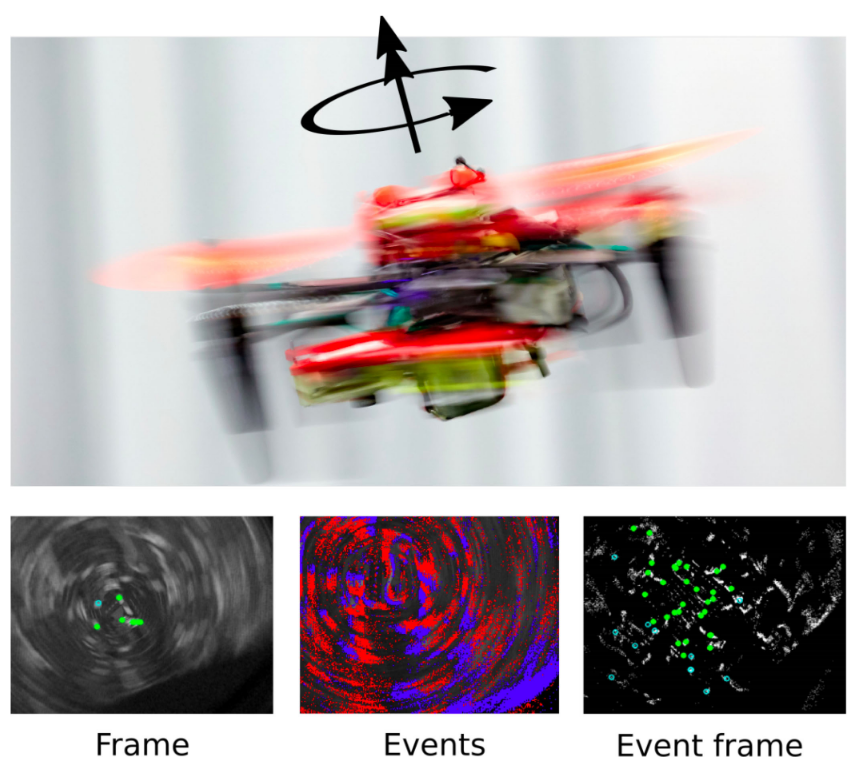
\includegraphics[width=0.65\textwidth]{02/sun-fail.png}}
\end{figure}

En investigación, técnicas de aprendizaje profundo han permitido dar un salto cuantitativo y cualitativo en las aplicaciones basadas en visión en la robótica aérea. Mejoras que tienen una aplicación directa en la seguridad, como la propuesta por S. Sun et al. con su algoritmo que evita un accidente en caso de fallo de un motor \cite{sun2021autonomous} (ver Fig. \ref{fig:sun}) o el algoritmo de evasión de obstáculos dinámicos desarrollado por D. Falanga et al \cite{falanga2020dynamic} (ver Fig. \ref{fig:falanga}).

\begin{figure}[ht]
 	\ffigbox[\FBwidth] {
 	    \caption[Secuencia de imágenes en maniobra de evasión]{Secuencia de imágenes en maniobra de evasión \cite{falanga2020dynamic}.}
 	    \label{fig:falanga}
 	}
 	{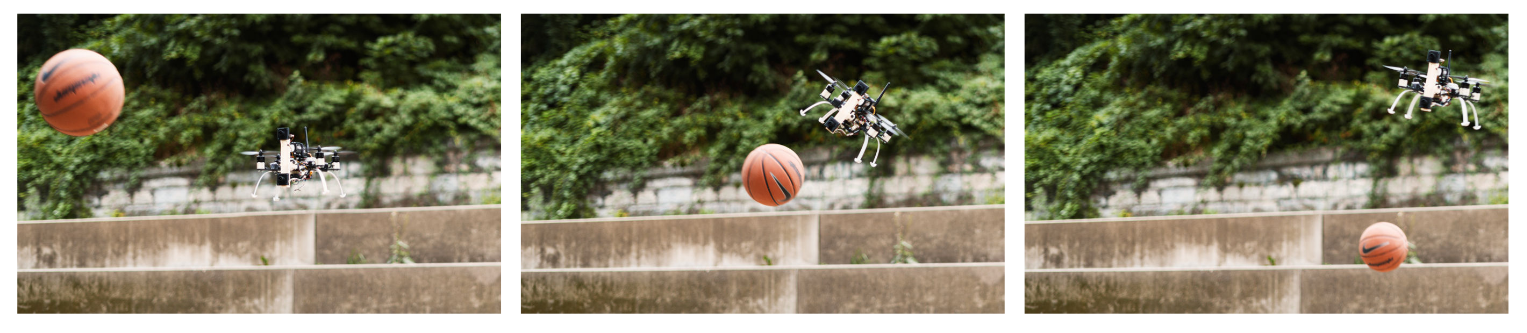
\includegraphics[width=0.95\textwidth]{02/falanga-avoidance.png}}
\end{figure}

Técnicas que han evolucionado de ser puramente de percepción a integrar también el control en la red neuronal. El algoritmo desarrollado por E. Kaufmann, \emph{Agile Drone Flight} \cite{kaufmann2018deep}, es prueba de ello. Este permite obtener posiciones y velocidades optimizadas a partir de una imagen utilizando redes neuronales profundas.  

Aeronaves como el Tello de DJI (Fig. \ref{fig:tello}) son ampliamente utilizadas en investigación debido a su bajo coste y tamaño. Ejemplo de ello puede ser el estudio realizado por A. Anwar y A. Raychowdhury donde proponen un nuevo algoritmo de navegación autónoma basado en técnicas de aprendizaje profundo \cite{anwar2020autonomous} o A. Scannell et al. en su investigación sobre nuevos algoritmos de optimización de trayectorias en entornos complejos \cite{scannell2021trajectory}.

% Davide Scaramuzza eth --> SVO
% Martin Saska prague

% enjambres Otra tendencia actual es la operación con un enjambre de aeronaves.  

% [1] EASA. Artificial Intelligence Roadmap: A human-centric approach to AI in aviation. Feb. 2020
% [2] Concepts of Design Assurance for Neural Networks (CoDANN) II

% https://etd.ohiolink.edu/apexprod/rws_etd/send_file/send?accession=ucin154409977396946&disposition=inline

\end{document}